\chapter[Resultados]{Resultados}
\label{result}

	Para cada \textit{shader} foram plotados os gráficos para as métricas relacionadas ao vértice e ao fragmento. Após as plotagens, percebeu-se que todos os gráficos de todos os \textit{shaders} relacionados ao vértice deram uma função linear (diferindo na inclinação), e os relacionados ao fragmento deram uma curva de formato semelhante. A Figura \ref{plotred} e a Figura \ref{plotrefl} mostram os gráficos plotados, com relação ao \textit{vertex} e \textit{fragment shaders} de cada \textit{shader} implementado, que demonstram a semelhança destas curvas

	 Os ajustes de cada curva (linear, exponencial, segundo e terceiro graus) também foram calculados e plotados (Figura \ref{linear} referente ao \textit{Reflection Shader}), em que também avisa-se qual foi o menor erro associado, a fim de descobrir qual a curva do \textit{fragment shader}. Pela a análise do menor erro, calculado de acordo com a Seção \ref{metminqua}, todos os \textit{shaders} indicaram uma curva de segundo grau.

	As equações calculadas para cada \textit{shader} (relacionadas ao vértice e fragmento) são mostradas na Tabela \ref{equacoes}. Assim, o processo utilizado neste trabalho, da análise da complexidade algorítimica calculada de forma empírica, pode ser resumido na Figura \ref{processo}. A etapa de Implementar \textit{Shaders} pode ser feita por meio da utilização da base do projeto implementado, extendendo-se da classe \textit{Shader} e implementando os métodos abstratos, como explicado na Seção \ref{imp}. A etapa Realização das Medições é feita de forma manual, dependendo do \textit{profiler} de GPU adequado para o \textit{device} utilizado. E a etapa Plotar Gráficos, Ajustar Curvas e Obter Equações é feita através do \textit{script} criado para o ajuste das curvas.

	\begin{figure}[ht]
	\centering
		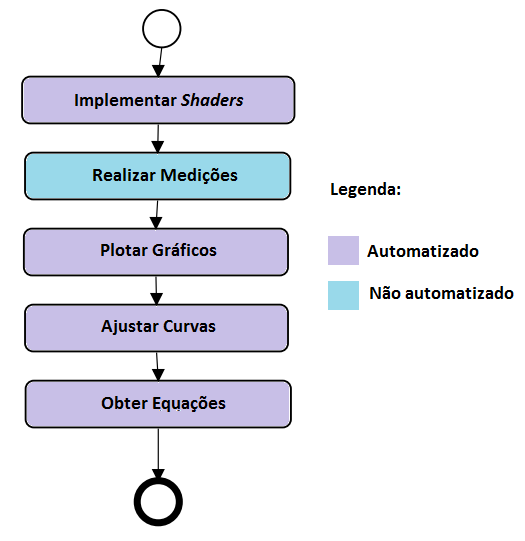
\includegraphics[keepaspectratio=true,scale=0.55]{figuras/processo.png}
	\caption{Processo da Análise de Complexidade Algorítmica.}
	\label{processo}
	\end{figure}

	\begin{figure}[ht]
	\centering
		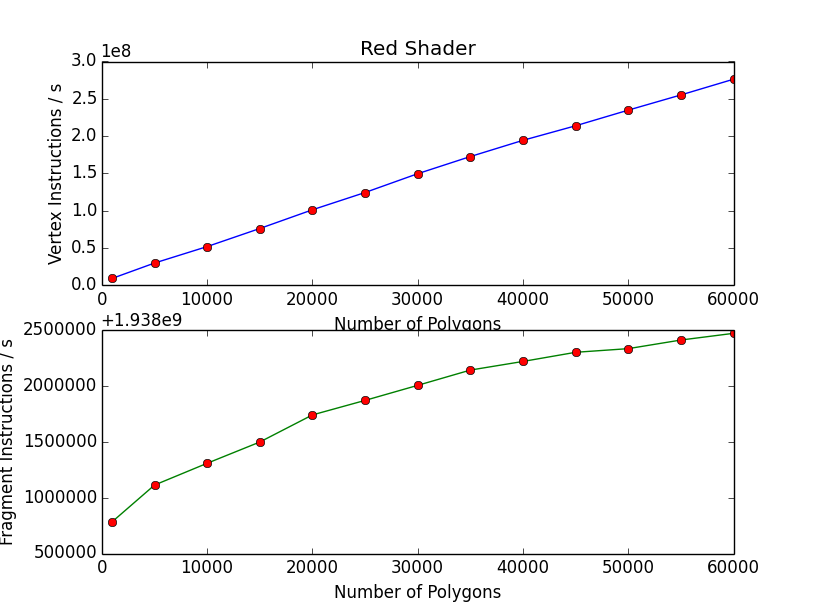
\includegraphics[keepaspectratio=true,scale=0.55]{figuras/red.png}
	\caption{Gráficos: \textit{Red Shader}, \textit{Toon shader}, \textit{Gouraud Shader},  \textit{Phong Shader} e  \textit{Flat Shader}}
	\label{plotred}
	\end{figure}

 
	\begin{figure}[ht]
	\centering
		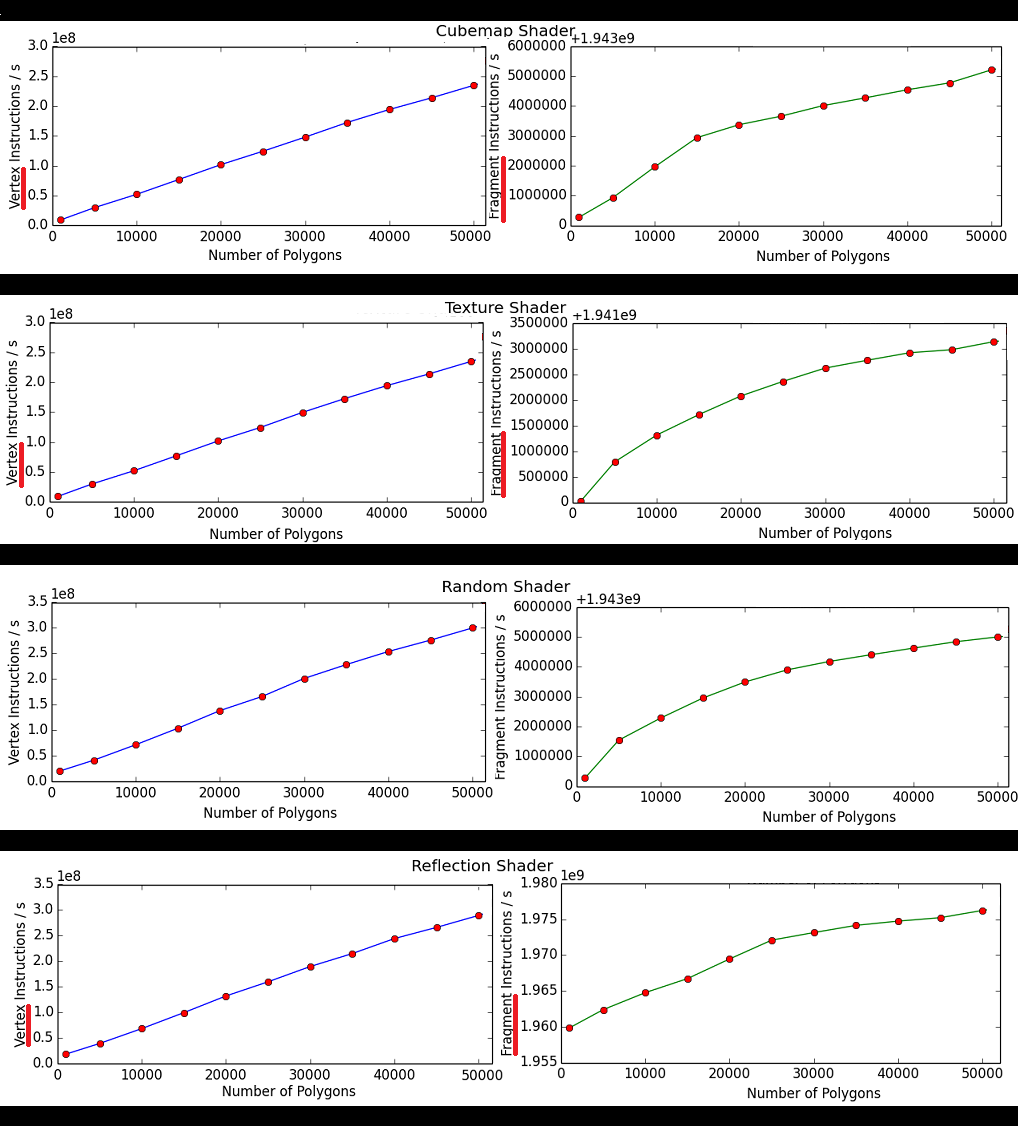
\includegraphics[keepaspectratio=true,scale=0.55]{figuras/cubeplot.png}
	\caption{Gráficos: \textit{Cubemap Shader}, \textit{Texture Shader}, \textit{Random Shader}, \textit{Reflection Shader}}
	\label{plotrefl}
	\end{figure}


	\begin{figure}[ht]
	\centering
		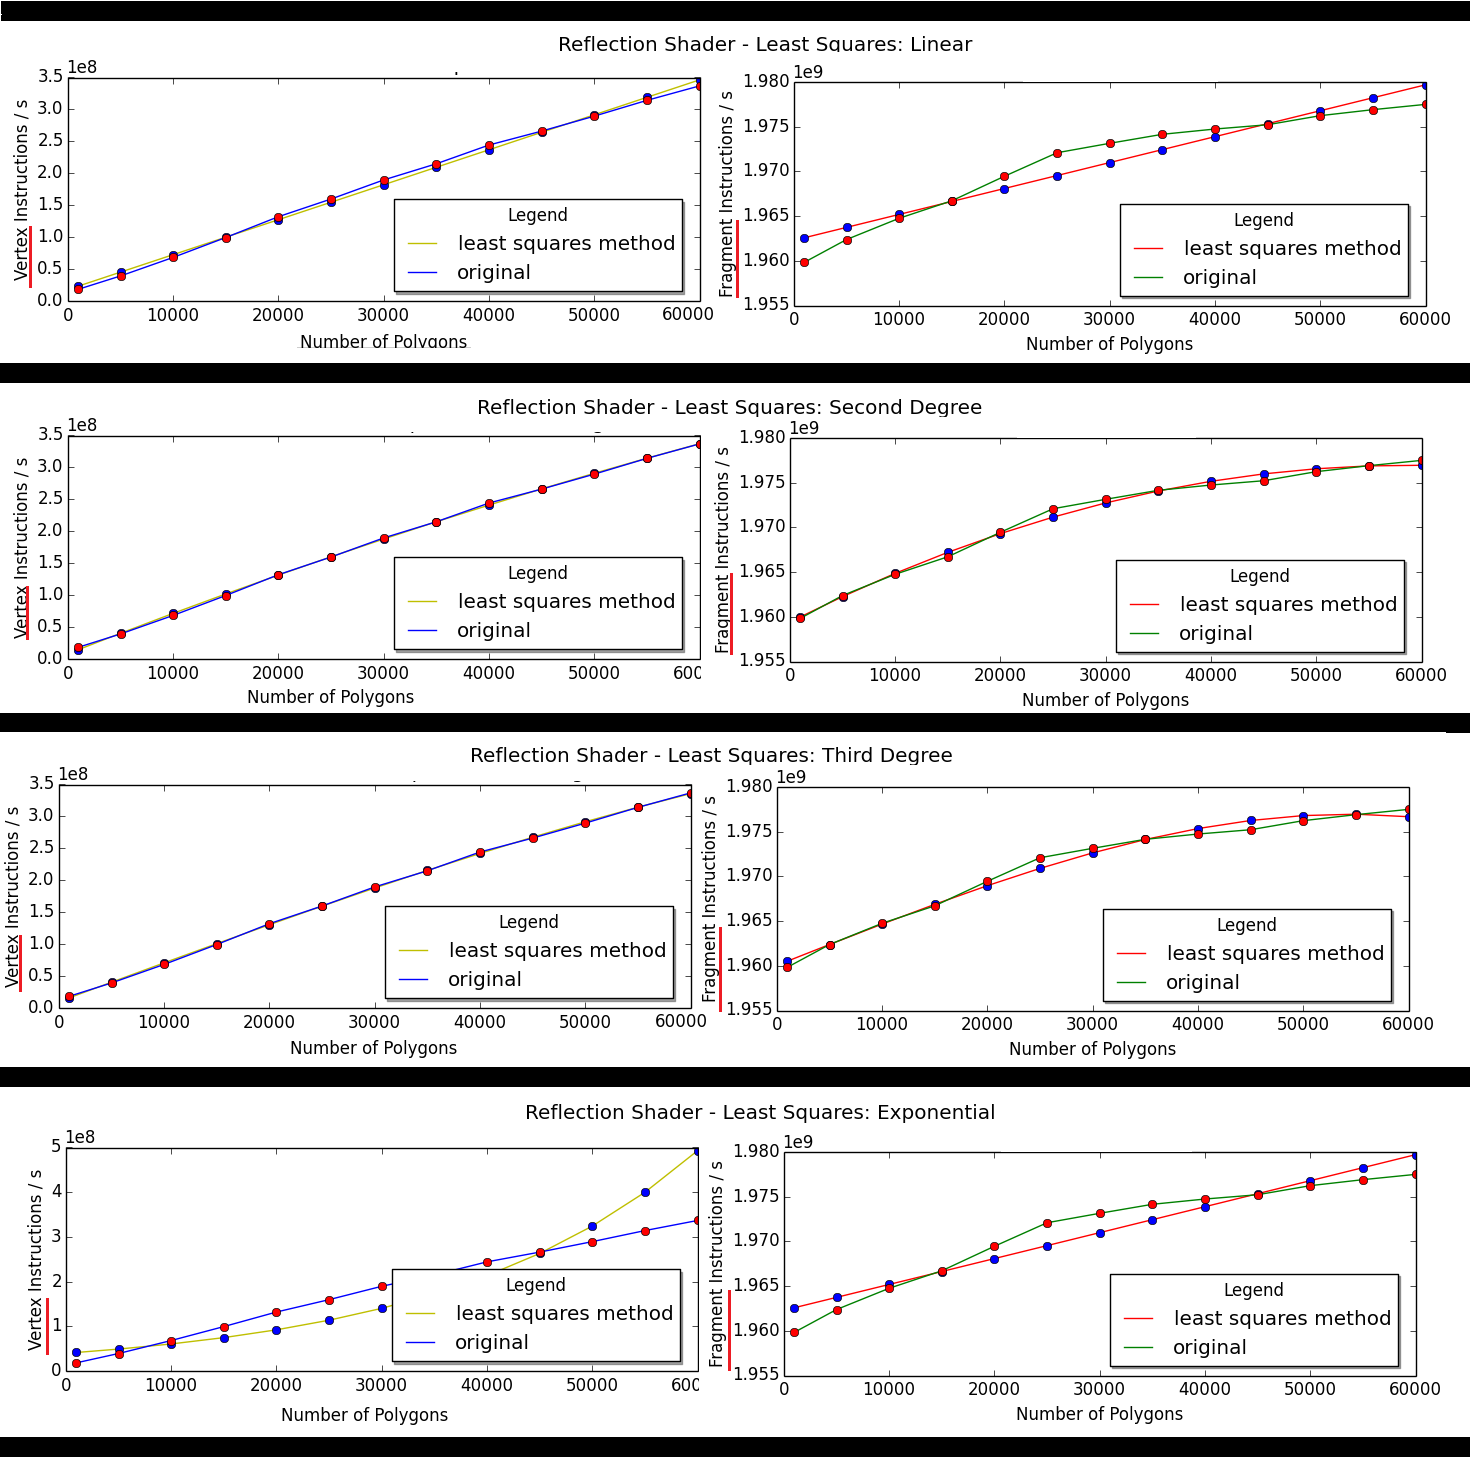
\includegraphics[keepaspectratio=true,scale=0.4]{figuras/reflectionlinear.png}
	\caption{Ajustes linear, para função de segundo, terceiro graus e exponencial}
	\label{linear}
	\end{figure}	
	

	\begin{table}[ht]
	\centering	
	\begin{tabularx}{0.9\textwidth}{cXX}
		\toprule
		\textbf{Nome} & \textbf{\textit{Equação Vertex Shader}} & \textbf{\textit{Equação Fragment Shader}}  \\
		\midrule
		\textit{Gouraud} & $y = 19.92 x 10^8 + 509.43t$ & $y = 67.99 x 10 ^5 + 6076.30t - 0.014t^2$ \\
		\textit{Phong} &  $y = 19.45 x 10^8 + 74.85t$ & $y = 20.20 x 10^6 + 9605.32t - 0.035t^2$\\
		\textit{Red} & $y = 19.39 x 10^8 + 26.84t$ & $y = 29.95 x 10 ^5 + 5130.50t - 0.0097t^2$ \\
		\textit{Toon} & $y = 19.45 x 10^8 + 100.35t$ & $y = 38.25 x 10 ^5 + 5347.86t - 0.011t^2$ \\
		\textit{Flat} & $y = 19.39 x 10^8 + 26.77t$ & $y = 25.02 x 10 ^5 + 4285.80t - 0.0091t^2$ \\
		\textit{Random Color} & $y = 19.45 x 10^8 + 74.04t$ & $y = 84.32 x 10 ^5 + 6930.50t - 0.021t^2$ \\
		\textit{Simple Texture} & $y = 19.42 x 10^8 + 49.97t$ & $y = 31.76 x 10 ^5 + 5137.26t - 0.0099t^2$ \\
		\textit{CubeMap} & $y = 19.44 x 10^8 + 83.38t$ & $y = 33.14 x 10 ^5 + 5109.61t - 0.0094t^2$ \\
		\textit{Reflection} & $y = 19.62 x 10^8 + 289.76t$ & $y = 83.92 x 10 ^5 + 6494.94t - 0.017t^2$ \\
	
		\bottomrule
	\end{tabularx}
	\caption{Equações relacionadas ao \textit{vertex shader} e \textit{fragment shader}}
	\label{equacoes}
	\end{table}
